\section{Auswertung}
\label{sec:Auswertung}

\subsection{Fehlerrechnung}
Die gemessenen Werte für Längen, Periodendauern und Massen werden im folgenden als nicht fehlerbehaftet 
angesehen. Die Fehler entstehen bei der bildung der Mittelwerte durch den Fehler des Mittelwertes und
bei der regressionsrechnung sowie der Fehlerfortpflanzung durch Python.

der Fehler des Mittelwertes beträgt
\begin{equation}
  \sqrt{\overline{x^2} - \overline{x}^2}
\end{equation}

Die Formel für die Feherfortpflanzung lautet
\begin{equation}
  \Delta f = \sqrt{\left(\frac{\partial f}{\partial x}\right)^2 \cdot \left(\Delta x\right)^2 + \left(\frac{\partial f}{\partial y}\right)^2 \cdot \left(\Delta y\right)^2 + .... + \left(\frac{\partial f}{\partial z}\right)^2 \cdot \left(\Delta z\right)^2}
\end{equation}



\subsection{Winkelrichtgröße D}
Im Folgenden wird zunächst die Winkelrichtgröße $D$ und das 
Eigenträgheitsmoment der Drehachse bestimmt. Dazu wird die
rücktreibende Kraft $F$ der Spiralfeder für verschiedene 
Auslenkungen $\varphi$ gemessen. \\
\begin{table}[H]
  \centering
  \caption{Messwerte zur Bestimmung von $D$.}
  \label{tab:tabelle}
  %\sisetup{table-format=1.1, per-mode=reciprocal}
  \begin{tblr}{
      colspec = {S S },
      row{1} = {guard, mode=math},
      %vline{4} = {2}{-}{text=\clap{$\pm$}},
    }
    \toprule
    \varphi(°) &  F(N)\\
    \midrule
    22.5  & 0\\
    45.0  & 0.04\\
    67.5  & 0.068\\
    90.0  & 0.09\\
    112.5 & 0.126\\
    135.0 & 0.164\\
    157.5 & 0.172\\
    180.0 & 0.18\\
    202.5 & 0.2\\
    225.0 & 0.28\\
   % \midrule
   % $\overline{\varphi}$ & $\overline{F}$\\
   % 123.75 & 0.132\\
   % \midrule
    \bottomrule
  \end{tblr}
\end{table}

Mithilfe von \eqref{eqn:gl9} und $r= 29,2cm$ kann die Winkelrichtgröße der 
Spiralfeder als Mittelwert von den errechneten
Größen für die einzelnen Messwerte zu %ich weiß nicht, was ich falsch mache, er will einfach nicht die gleichung im pdf referenzieren.
0.00002790 \pm 0.000003259 $\frac{N \cdot m}{rad}$ bestimmt werden. 

\subsection{Eigenträgheitsmoment $I_D$}
Als nächstes wird das Eigenträgheitsmoment $I_D$ der Drillachse bestimmt.
 
\begin{equation}
  I_{ges} = I_D + I_s + 2\cdot(I_z + m_z \cdot a^2)
\end{equation}

\begin{equation}
  I_{ges} = I_D + \frac{ml^2}{12} + 2\cdot m_z \cdot \left(\left(\frac{r^2}{4} + \frac{h^2}{12} \right) + \cdot a^2\right)
\end{equation}

Durch einsetzen in \autoref{eqn:gl10} und aus der umgestelten Geradengleichung
\begin{equation}
  b = y - m \cdot x
\end{equation}
ergibt sich die gleichung für das Eigenträgheitsmoment $I_D$
\begin{equation}
  \label{eqn:Id}
  I_D = \frac{bD}{4\pi^2} - \left(2\cdot m_z \cdot \left(\frac{r^2}{4} + \frac{h^2}{12} \right) + \frac{m_s\cdot l_s}{12}\right)
\end{equation}


 \begin{table}[H]
   \centering
   \caption{Messwerte T/a.}
   \label{tab:at}
   %\sisetup{table-format=1.1, per-mode=reciprocal}
   \begin{tblr}{
       colspec = {S S },
       row{1} = {guard, mode=math},
       %vline{4} = {2}{-}{text=\clap{$\pm$}},
     }
     \toprule
     a(cm) & T(s)\\
     \midrule
     10    & 3.28\\
     11.5  & 3.71\\
     13    & 4.28\\
     14.5  & 4.75\\
     16    & 5.25\\
     17.5  & 5.90\\
     19    & 6.28\\
     20.5  & 6.78\\
     22    & 7.28\\
     23.5  & 7.97\\
     \midrule
     $\overline{T}$ & $\overline{a}$\\
     \midrule
     \bottomrule
   \end{tblr}
 \end{table}

 %messwerte zur berechnng von ID
 \begin{table}[H]
  \centering
  \caption{Messwerte zur berechnung von $I_D$}
  \label{tab:messwerteId}
  %\sisetup{table-format=1.1, per-mode=reciprocal}
  \begin{tblr}{
      colspec = {S S S S S },
      row{1} = {guard, mode=math},
      row{2} = {guard, mode=math},
      row{14} = {guard},
      %vline{4} = {2}{-}{text=\clap{$\pm$}},
    }
    \toprule
    m_{Zylinder}(kg) & r_{Zylinder}(m)  & h_{Zylinder}(m) & m_{Stab} (kg)& l_{Stab}(m) \\
    \midrule
    0.219 & 0.017 & 0.03 & 0.1 & 0.6  \\
    \bottomrule
  \end{tblr}
\end{table}

Als Masse des Stabes haben wir 0.1 gk angenommmen, da wir ihn nicht gewogen haben.

\begin{figure}[H]
  \centering
  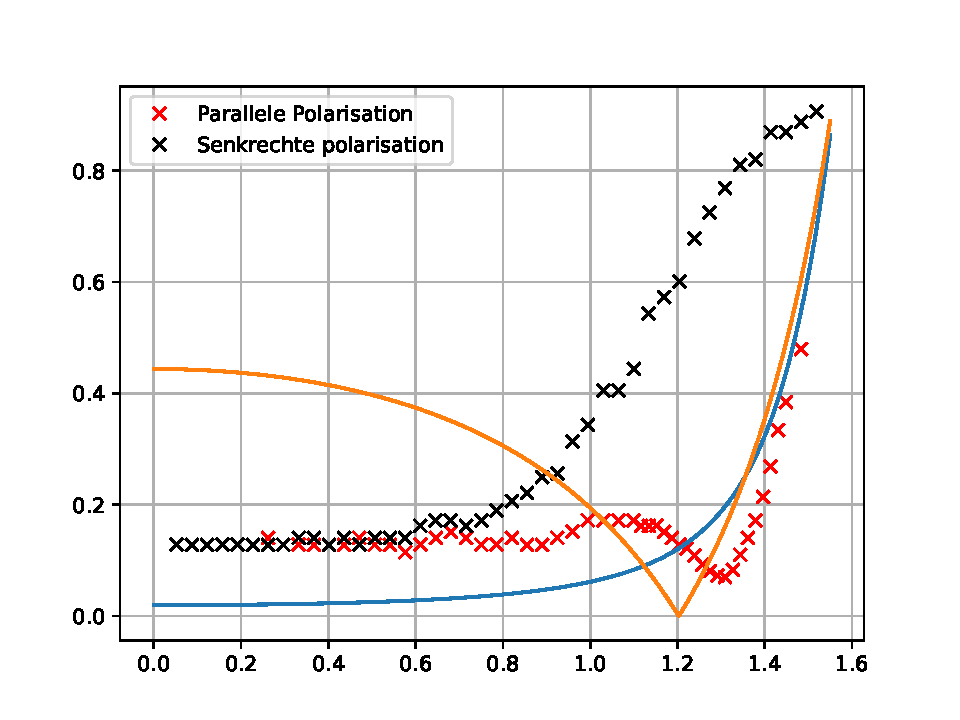
\includegraphics{plot.pdf}
  \caption{Lineare Regression zur bestimmung von $I_D$.}
  \label{fig:linreg}
\end{figure}

Die Messwerte der Periodendauer in abhängigkeit von dem Abstand der Gewichte sind 
der \autoref{tab:at} zu entnehmen. Daraus ergibt sich die Liniare Regression\autoref{fig:linreg}.
die Parameter der Ausgleichsgeraden sind $m = 113.343 \pm 1.623 $ und $ b = -1.019 \pm 0.540$.
Daraus folgt durch Einseten des Parameters b und den Messwerten aus \autoref{tab:messwerteId} in \autoref{eqn:Id}
\begin{center}
$I_D = -0.005072\pm0.000004$ 
\end{center}

\subsection{Trägheitsmoment Kugel und Zylinder}
%Kugel
\begin{table}[H]
  \centering
  \caption{Abmessungen Holzkugel.}
  \label{tab:kugel}
  %\sisetup{table-format=1.1, per-mode=reciprocal}
  \begin{tblr}{
      colspec = {S S },
      row{1} = {guard, mode=math},
      %vline{4} = {2}{-}{text=\clap{$\pm$}},
    }
    \toprule
    r(m) & m(kg)\\
    \midrule
    0.0605\pm 0.0001  & 0.638\pm 0.001 \\
    \bottomrule
  \end{tblr}
\end{table}
%zylinder
\begin{table}[H]
  \centering
  \caption{Abmessungen Holzzylinder.}
  \label{tab:zylinder}
  %\sisetup{table-format=1.1, per-mode=reciprocal}
  \begin{tblr}{
      colspec = {S S S},
      row{1} = {guard, mode=math},
      %vline{4} = {2}{-}{text=\clap{$\pm$}},
    }
    \toprule
    r(m) & h(m) & m(kg)\\
    \midrule
    0.0493\pm 0.0001 & 0.0995\pm 0.0001 & 0.366\pm 0.001 \\
    \bottomrule
  \end{tblr}
\end{table}

Hier sollte das Trägheitsmoment von einer Kugel und eines Zylinders berechnet werden. mit den maßen aus \autoref{tab:kugel}
und \autoref{eqn:gl5} berechnet sich $I_{Holzkugel} = (0.0009350\pm0.0000034)kg ⋅ m²$ sowie das Trägheitsmoment des Zylinders
mit den Abmessungen \autoref{tab:zylinder} eingesetzt in \autoref{eqn:gl6} berechnet sich zu $I_Holzzylinder = 
0.000444\pm0.0000022 kg ⋅ m²$.

\subsection{Experimentelles Trägheitsmoment Kugel}
Dann wird wie in \autoref{sec:zwei körper} das System zum Schwingen gebracht und die Periodendauer 
dokumentiert. Daraus berechnet man mit Hilfe der \autoref{equ:gl10} nach dem Trägheitsmoment I umgestellt zu
\begin {equation}
\label{eqn:gl11}
\frac{T^2}{4*\pi^2}*D = \symbf{I}
\end{equation}
das experimentelle Trägheitsmoment der Kugel. Identische Vorgehensweise ebenfalls beim Zylinder.

%Messwerte T Kugel
\begin{table}[H]
  \centering
  \caption{Schwingungsdauer Kugel}
  \label{tab:Tkugel}
  %\sisetup{table-format=1.1, per-mode=reciprocal}
  \begin{tblr}{
      colspec = {S S},
      row{1} = {guard, mode=math},
      %vline{4} = {2}{-}{text=\clap{$\pm$}},
    }
    \toprule
    T_k(s) Kugel & T_Z(s) Zylinder\\
    \midrule
    1.13 & 0.78\\
    1.22 & 0.65\\
    1.15 & 0.78\\
    1.16 & 0.78\\
    1.16 & 0.78\\
    1.22 & 0.75\\
    1.22 & 0.72\\
    1.25 & 0.79\\
    1.16 & 0.75\\
    1.19 & 0.78\\
    \midrule
    $\overline{T_k}$ & $\overline{T_z}$\\
    \midrule
    1.186 \pm 0.0124 & 0.756 \pm 0.0135\\
    \bottomrule
  \end{tblr}
\end{table}

bei Berücksichtigung der Mittelwerte und dem zugehörigen Standardehler des Mittelwerts beläuft 
sich das Trägheitsmoment für die Kugel auf $I_k = (0.00097 \pm 0.00011)$ und das Trägheitsmoment 
des Zylinders auf $I_z = (0.00039 \pm 0.00005)$.


\subsection{Trägheitsmoment von zwei Puppen}
Um das theoretische Trägheitsmoment einer Puppe in ihrer eingenommenen 
Position zu berechnen, benötigt man die Abmessungen der einzelnen Körperteile, 
sowie deren Masse, Ausrichting und die Entfernung von der Rotationsachse. 
Zunächst haben wir die Volumina der Einzelkörperteile der Puppe bestimmt. Wenn man diese Teilvolumina 
durch das Gesamtvolumen der Puppe teilt, erhält man den Anteil der Masse des Volumenstückes 
an der Gesamtmasse. So kann man alle Größen vereinfacht angeben und zur theoretischen Berechnung nutzen.



\begin{table}[H]
  \centering
  \caption{Abmessungen Puppe}
  \label{tab:maßePuppe}
  %\sisetup{table-format=1.1, per-mode=reciprocal}
  \begin{tblr}{
      colspec = {S S S S S},
      row{1} = {guard, mode=math},
      row{14} = {guard},
      %vline{4} = {2}{-}{text=\clap{$\pm$}},
    }
    \toprule
    \SetCell[c=2]{c} R_{Arme}(cm) & & R_{Beine}(cm) & R_{Torso}(cm) & R_{Kopf}(cm)\\
    \midrule
    0.985  &0.875 & 1.25   &  1.885  & 1.580\\
    0.925  &0.905 & 1.305  &  2.415  & 1.725\\
    1.045  &0.95  & 1.19   &  2.195  & 1.715\\
    1.055  &0.91  & 1      &  2.03   & 1.65\\
    1.05   &0.81  & 0.95   &  3.67   & 1.59\\
    0.995  &0.775 & 1.010  &  2.14   & 1.425\\
    0.88   &0.71  & 1.075  &  2.485  & \\
    0.8    &0.655 & 0.97   &  2.495  & \\
    0.795  &0.8   & 0.825  &  2.36   & \\
    0.79   &1.95  & 0.78   &  1.925  & \\
    \midrule
    &$\overline{R_A}$  & $\overline{R_B}$ & $\overline{R_T}$ & $\overline{R_K}$\\
    \midrule
    \SetCell[c=2]{c} 0.93\pm0.06 & &  1.04\pm0.05 &  3.93\pm0.16 & 1.61\pm0.05  \\
    \midrule
    \SetCell[c=2]{c}$h_A$ (cm)&& $h_B$ (cm)& $h_T$ (cm)& $h_K$(cm)\\
    \midrule
    \SetCell[c=2]{c} 11.81 && 16.0 & 11.47 & 5.02\\
    \bottomrule
  \end{tblr}
\end{table}

In der \autoref{tab:maßePuppe} sind die gemittelten Radien und die Höhen der Körperteile 
aufgeführt. (Am Anfang ein bisschen übertriebene 20 Messwerte). wir Teilen die Puppe in ihre 
sechs Körperteile ein, welche alle als Zylinder genähert werden. Also können wir die Volumina 
der Körperteile mit folgender Formel berechnen

\begin{equation}
  \symbf{V} = h * \pi * r^2
\end{equation}

\begin{table}[H]
  \centering
  \caption{Volumina Körperteile}
  \label{tab:Volumina}
  %\sisetup{table-format=1.1, per-mode=reciprocal}
  \begin{tblr}{
      colspec = {S S S S },
      row{1} = {guard, mode=math},
      row{14} = {guard},
      %vline{4} = {2}{-}{text=\clap{$\pm$}},
    }
    \toprule
     V_{Arme}(cm³)  & V_{Beine}(cm³) & V_{Torso}(cm³) & V_{Kopf}(cm³)\\
    \midrule
    54\pm6  &54\pm6    &  557.48 \pm 45.82  &  41.1\pm2.3\\
    \bottomrule
  \end{tblr}
\end{table}

Daraus bestimmen wir die Masse der Körperteile

\begin{equation}
  m_{i} = m_{gesamt} * \frac{V_i}{Vg}
\end{equation}

\begin{table}[H]
  \centering
  \caption{Massen Körperteile}
  \label{tab:Massen}
  %\sisetup{table-format=1.1, per-mode=reciprocal}
  \begin{tblr}{
      colspec = {S S S S },
      row{1} = {guard, mode=math},
      row{14} = {guard},
      %vline{4} = {2}{-}{text=\clap{$\pm$}},
    }
    \toprule
     m_{Arme}(g)  & m_{Beine}(g) & m_{Torso}(g) & m_{Kopf}(g)\\
    \midrule
    25.2\pm2.8  &25.2\pm2.8    &  261 \pm 6  & 19.2\pm1.6\\
    \bottomrule
  \end{tblr}
\end{table}

und daraus mithilfe von \autoref{eqn:gl6} und \autoref{eqn:gl7} die Teilträgheitsmomente 
um ihre eigene jeweilige Drehachse.

\begin{table}[H]
  \centering
  \caption{Teilträgheitsmomente}
  \label{tab:Trägheitsmomente}
  %\sisetup{table-format=1.1, per-mode=reciprocal}
  \begin{tblr}{
      colspec = {S S S S S S},
      row{1} = {guard, mode=math},
      row{2} = {guard, mode=math},
      row{14} = {guard},
      %vline{4} = {2}{-}{text=\clap{$\pm$}},
    }
    \toprule
     I_a (g \cdot cm^2)& I_{aHorizontal}(g \cdot cm^2) & I_b(g \cdot cm^2) & I_{bHorizontal} (g \cdot cm^2)& I_t (g \cdot cm^2)& I_k (g \cdot cm^2)& \\
    \midrule
    8.8\pm1.5  &  299\pm33 & 10.8\pm2.2  & 545 \pm 60& 1615 \pm 162& 20.1\pm2.6  \\
    \bottomrule
  \end{tblr}
\end{table}

Damit haben wir alle Größen um das theoretische Trägheitsmoment der Puppen in 
Pos1 \autoref{fig:pos1} und Pos2 \autoref{fig:pos2} zu bestimmen. 

Für die Arme und Beine wird der Satz von Steiner verwendet \autoref{eqn:steiner} um die Drehachse der 
Trägheitsmomente von den einzelnen Körperteile in die Drehachse der Puppe zu legen. In der 
Position eins wird der Abstand der Eigendrehachse der Beine zur Drehachse der Puppe mit 
dem Radius der Beine genähert, sowie der Abstand der Arme zur Drehachse der Puppe mit dem Radius der Arme 
und dem Radius des Torso. In der ersten Position ist der Abstand zur Achse des Arms: der Radius des torso 
und die halbe Armlänge. Der Abstand des ausgestrekten Beins ist die halbe Beinlänge.

\begin{equation}
  \label{eqn:steiner}
  I_{neu} = I + m * r^2
\end{equation}

Damit ergeben sich die theoretischen Trägheitsmomente zu
\begin{center}
  $I_{pos1} = 0.000292 \pm 0.000018  kg \cdot m^2$
\end{center}
\begin{center}
  $\symbf{I}_{pos2} = 0.001090 \pm 0.000085  kg \cdot m^2$
\end{center}

\subsection{Experimentelles Trägheitsmoment von zwei Puppen}
 Nun werden die Trägheitsmomente noch einmal experimentell bestimmt.

 \begin{table}[H]
  \centering
  \caption{Schwingungsdauer der Puppe}
  \label{tab:Tpuppe}
  %\sisetup{table-format=1.1, per-mode=reciprocal}
  \begin{tblr}{
      colspec = {S S},
      row{1} = {guard, mode=math},
      %vline{4} = {2}{-}{text=\clap{$\pm$}},
    }
    \toprule
    T_k(s) pos1 & T_Z(s) pos2\\
    \midrule
    0.75 & 1.59\\
    0.82 & 1.63\\
    0.78 & 1.75\\
    0.84 & 1.69\\
    0.72 & 1.65\\
    0.78 & 1.78\\
    0.78 & 1.72\\
    0.88 & 1.61\\
    0.78 & 1.62\\
    0.85 & 1.55\\
    \midrule
    $\overline{T_{pos1}}$ & $\overline{T_{pos2}}$\\
    \midrule
    0.797 \pm 0.015 & 1.659 \pm 0.023\\
    \bottomrule
  \end{tblr}
\end{table}

Aus den Mittelwerten ergibt sich nach \autoref{eqn:gl11}
\begin{center}
$\symbf{I}_{expPos1} = 0.00044\pm0.00005  kg \cdot m^2$
\end{center}
\begin{center}
  $\symbf{I}_{expPos1} = 0.00189\pm0.00023  kg \cdot m^2$
\end{center}



